% Results, per-class, ensemble, importances
\section{Results}

\begin{frame}{Overall Results on 1{,}635 Held-Out Events}
  \begin{columns}[T]
    \begin{column}{0.54\textwidth}
      \centering\small
      \setlength{\tabcolsep}{4pt}
      \begin{tabular}{lccc}
        \toprule
        Model & Acc. & Macro-F1 & Wtd-F1 \\
        \midrule
        LightGBM         & 0.9223 & \good{0.6949} & 0.9148 \\
        XGBoost          & 0.9168 & 0.6906 & 0.9114 \\
        MLP-NN           & 0.9242 & \bad{0.5843} & 0.8992 \\
        TabNet           & \amb{0.9254} & 0.6027 & 0.9020 \\
        Stacked Ensemble & 0.8948 & 0.6639 & 0.8968 \\
        \bottomrule
      \end{tabular}

      \vspace{3mm}
      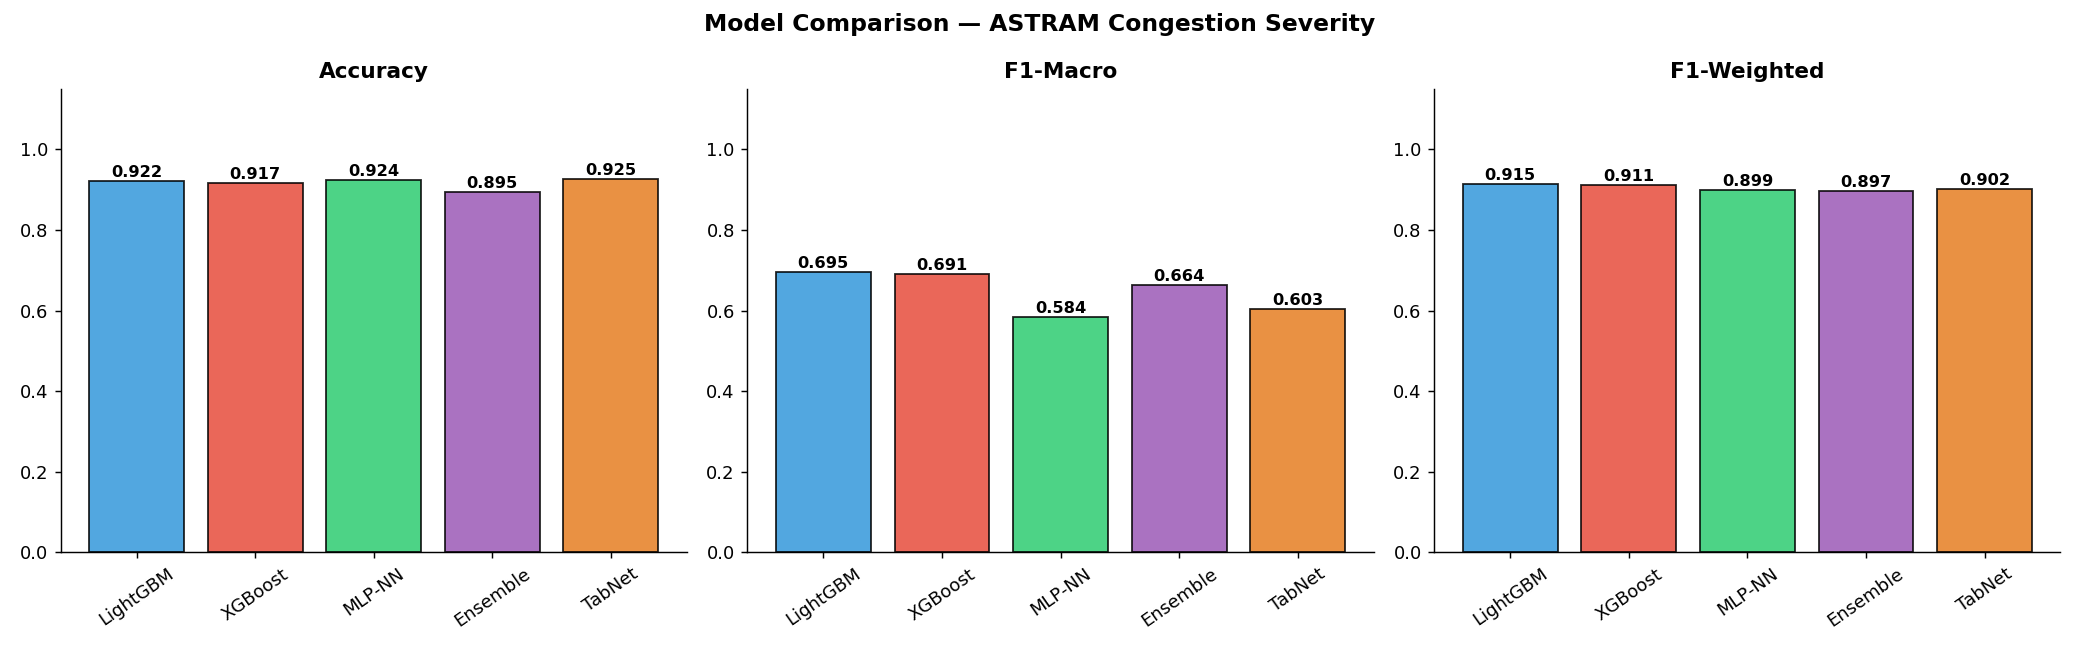
\includegraphics[width=0.95\textwidth]{figs/model_comparison.png}
    \end{column}
    \begin{column}{0.44\textwidth}
      \begin{block}{A narrow accuracy band}
        \small Every model sits between 89\% and 93\% accuracy, a spread that
        looks unremarkable. Macro-F1 ranges from 0.5843 to 0.6949, a gap far too
        wide to be explained by those near-identical accuracies.
      \end{block}
      \begin{alertblock}{The reversal}
        \small TabNet posts the \textbf{highest accuracy}. LightGBM has the
        \textbf{best macro-F1}. Ranking these models by accuracy would point a
        deployment decision at the wrong model.
      \end{alertblock}
    \end{column}
  \end{columns}
\end{frame}

\begin{frame}[shrink=5]{Per-Class Results: Where the Spread Comes From}
  \begin{columns}[T]
    \begin{column}{0.48\textwidth}
      \centering
      \textbf{Critical class} (support $=$ 59)\\[1mm]
      \begin{tabular}{lccc}
        \toprule
        Model & Prec. & Recall & F1 \\
        \midrule
        LightGBM         & 0.54 & 0.32 & \good{0.40} \\
        XGBoost          & 0.46 & \good{0.36} & \good{0.40} \\
        MLP-NN           & 1.00 & \bad{0.03} & \bad{0.07} \\
        TabNet           & 0.75 & \bad{0.10} & 0.18 \\
        Stacked Ensemble & 0.28 & 0.34 & 0.31 \\
        \bottomrule
      \end{tabular}

      \vspace{3mm}
      \textbf{Medium class} (support $=$ 76)\\[1mm]
      \begin{tabular}{lccc}
        \toprule
        Model & Prec. & Recall & F1 \\
        \midrule
        LightGBM         & 0.58 & 0.39 & \good{0.47} \\
        XGBoost          & 0.56 & 0.39 & 0.46 \\
        MLP-NN           & 0.75 & 0.24 & 0.36 \\
        TabNet           & 0.83 & 0.20 & \bad{0.32} \\
        Stacked Ensemble & 0.49 & \good{0.46} & \good{0.47} \\
        \bottomrule
      \end{tabular}
    \end{column}
    \begin{column}{0.5\textwidth}
      \begin{exampleblock}{Key finding}
        \small The only two models with \emph{usable} Critical recall,
        LightGBM (0.32) and XGBoost (0.36), are \textbf{exactly the two
        trained with class-balanced weighting}.
      \end{exampleblock}
      \begin{block}{Majority classes are easy}
        \small Every model handles Low (F1 0.93--0.94) and High (F1 0.95--0.97)
        comfortably. The entire macro-F1 spread comes from the two rare classes
        exactly what accuracy hides.
      \end{block}
      \begin{alertblock}{Honest note on stacking}
        \small The ensemble posts the \emph{lowest} accuracy of the five
        (0.8948). Its in-fold models were lighter, and each fold holds under
        100 rare-class examples. It still reaches the second-best Critical
        recall.
      \end{alertblock}
    \end{column}
  \end{columns}
\end{frame}



\begin{frame}[shrink]{Feature Importances}
  \begin{columns}[T]
    \begin{column}{0.52\textwidth}
      \centering
      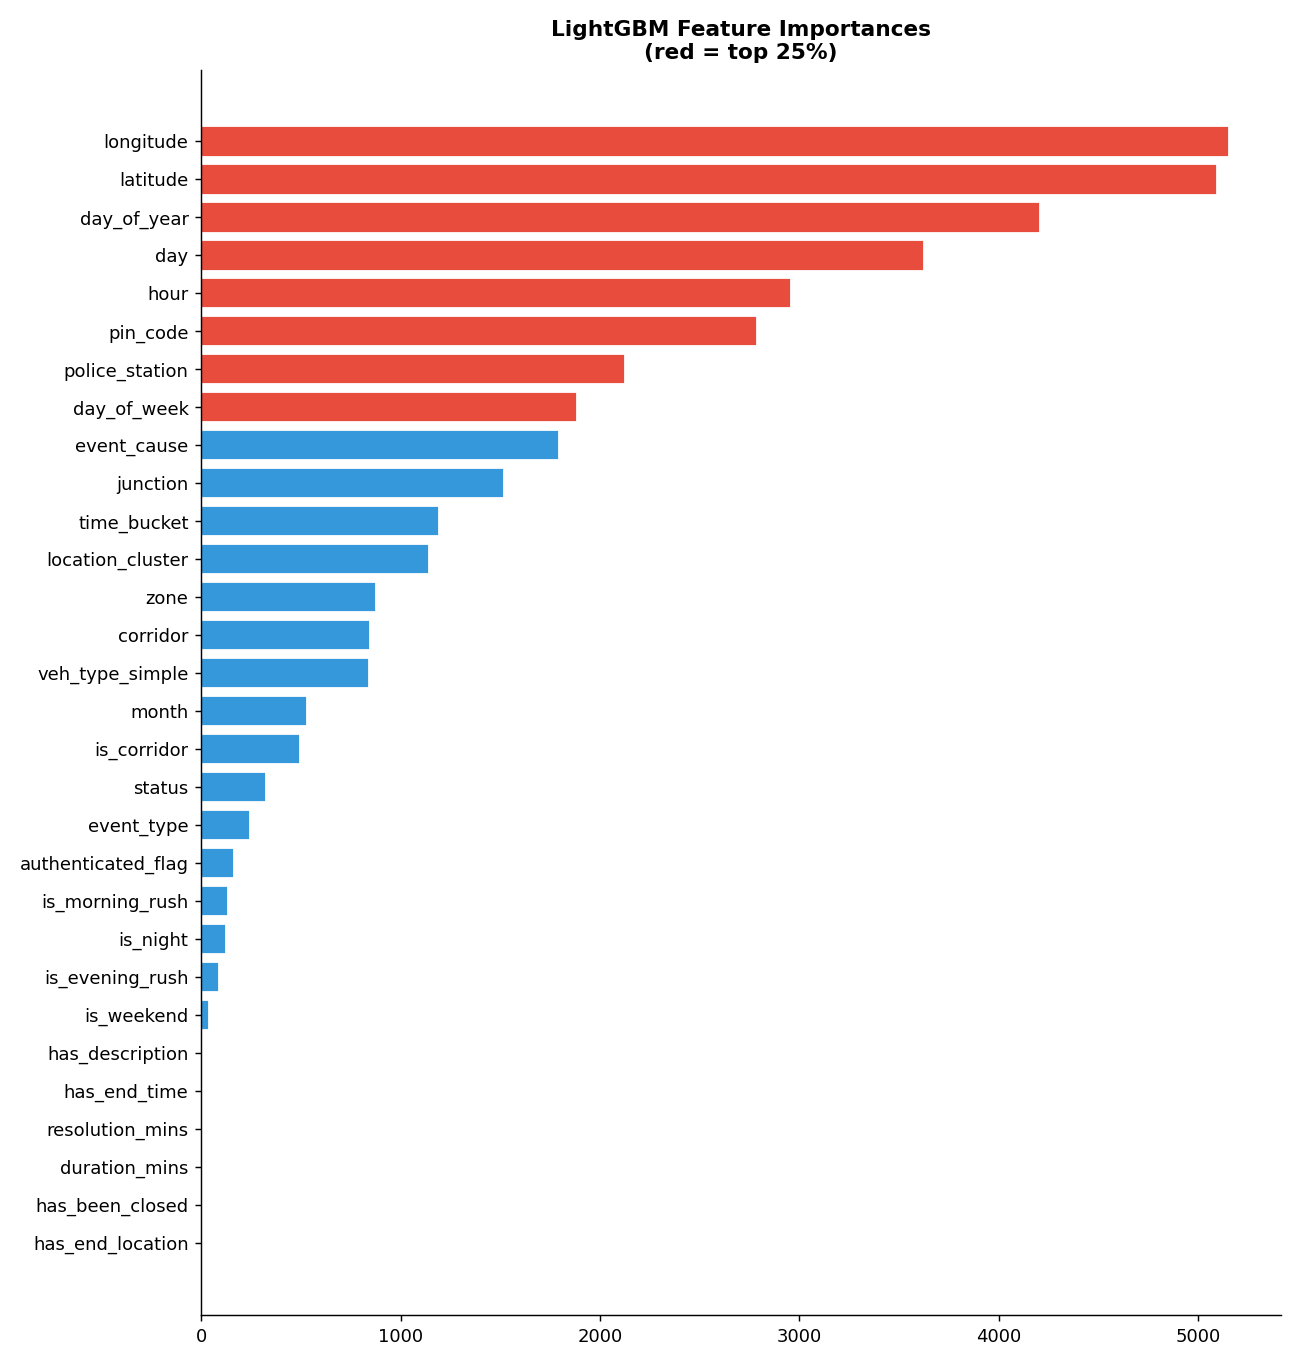
\includegraphics[width=\textwidth]{figs/lgbm_feature_importance.png}\\
      {\scriptsize LightGBM split-based importance; red bars mark the top
      quartile.}
    \end{column}
    \begin{column}{0.46\textwidth}
      \begin{block}{What ranks highest}
        \small
        \begin{itemize}
          \item \textbf{Raw coordinates dominate}: \texttt{longitude} and
                \texttt{latitude} are the two most-used split features.
          \item \textbf{Fine-grained time next}: \texttt{day\_of\_year},
                \texttt{day}, \texttt{hour}.
          \item \textbf{Then jurisdiction and cause}: \texttt{pin\_code},
                \texttt{police\_station}, \texttt{day\_of\_week},
                \texttt{event\_cause}.
        \end{itemize}
      \end{block}
      \begin{alertblock}{Caveat}
        \small Split-count importance favours \textbf{high-cardinality}
        features. That is why the engineered binary flags
        (\texttt{is\_corridor}, \texttt{is\_weekend}, rush-hour) sit at the
        bottom: it counts how \emph{often} a feature is split on, not the size or
        direction of its effect.
      \end{alertblock}
    \end{column}
  \end{columns}
\end{frame}

% =====================================================================
